

\begin{figure}
\begin{subfigure}{.5\linewidth}
\centering

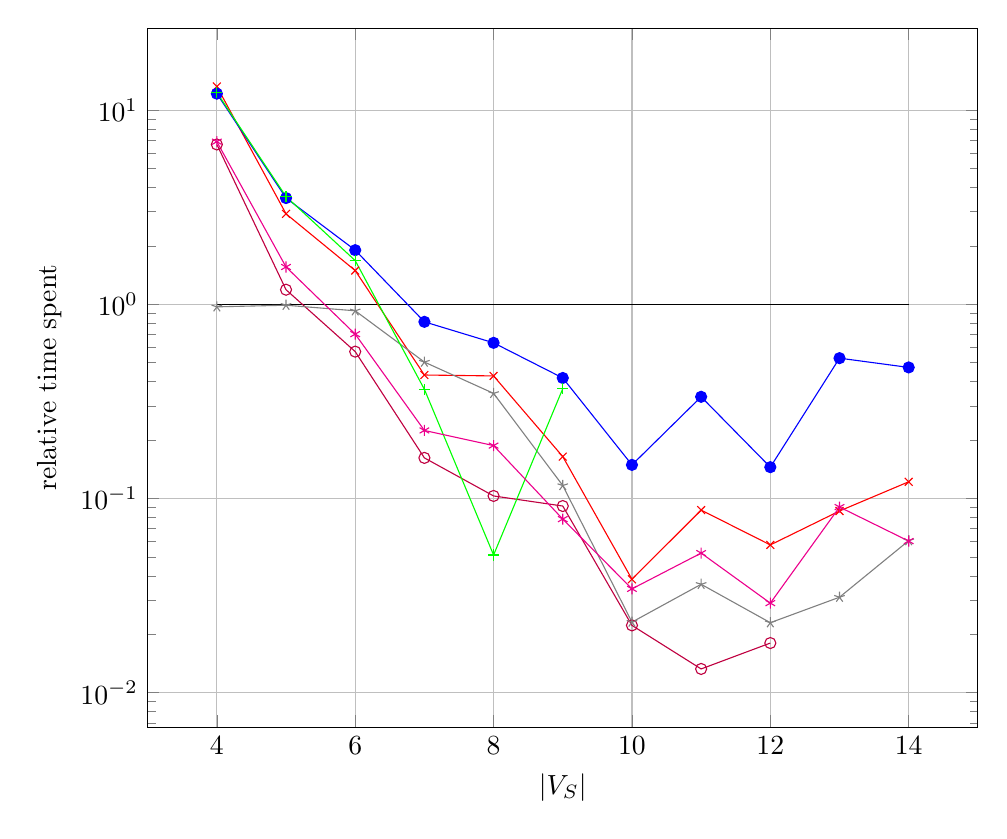
\begin{tikzpicture}
    \begin{axis}[
        xlabel=$|V_S|$,
        ylabel=relative time spent,
        ymode=log,
        legend style={at={(0.9,0.1)},anchor=south east},
        width=\textwidth,
		y tick label style={/pgf/number format/sci},
        ymajorgrids,
        xmajorgrids,		
    ]
\addplot [mark=none, black] plot coordinates {
        (4,1) (14, 1)};

    
	

\addplot[
        mark=x,
        red,
    ] plot coordinates {
        (4,13.228536748772864)
        (5,2.923043265236232)
        (6,1.4918465046685692)
        (7,0.43251422608381307)
        (8,0.4278138461953538)
        (9,0.1643974532055621)
        (10,0.0384235218883735)
        (11,0.08720339702951019)
        (12,0.05769871433439522)
        (13,0.08626318052038495)
        (14,0.12196687793734029)
};
%    \addlegendentry{DFS}


\addplot[
        mark=o,
        purple,
    ] plot coordinates {
        (4,6.652084765296219)
        (5,1.1887666847267304)
        (6,0.5706904469839822)
        (7,0.1619203743990465)
        (8,0.10311284594841497)
        (9,0.09148726872328639)
        (10,0.02222929883828284)
        (11,0.013264269229998682)
        (12,0.01803108077997606)
};
%    \addlegendentry{GDFS O IP}


\addplot[
        mark=star,
        gray,
    ] plot coordinates {
        (4,0.9704520516781957)
        (5,0.9891315449448252)
        (6,0.9259991321183858)
        (7,0.5041146272686665)
        (8,0.34789464456875185)
        (9,0.11668758068736773)
        (10,0.023108258037857765)
        (11,0.03619415549870497)
        (12,0.022948727466520213)
        (13,0.031049777535341994)
        (14,0.06069360971979865)
};
%    \addlegendentry{GDFS C}


\addplot[
        mark=*,
        blue,
    ] plot coordinates {
        (4,12.149621156018027)
        (5,3.524039042210963)
        (6,1.9000540945545796)
        (7,0.8124353858557827)
        (8,0.6333558749485183)
        (9,0.4176331133841372)
        (10,0.1490144308922331)
        (11,0.33404804566046264)
        (12,0.14504260141405623)
        (13,0.5281107544448288)
        (14,0.4731679498288802)
};
%    \addlegendentry{K-Path}


\addplot[
        mark=+,
        green,
    ] plot coordinates {
        (4,12.32026911652997)
        (5,3.58755573944772)
        (6,1.6790110096274846)
        (7,0.36496009660452833)
        (8,0.05120848928373445)
        (9,0.3680142027878651)
};
%    \addlegendentry{CP}


\addplot[
        mark=asterisk,
        magenta,
    ] plot coordinates {
        (4,6.876029334720606)
        (5,1.556841256929411)
        (6,0.7022607700874779)
        (7,0.22412843275278505)
        (8,0.18733394302820017)
        (9,0.07837119253519409)
        (10,0.03427027564684937)
        (11,0.05237617390308613)
        (12,0.028947697493439506)
        (13,0.09038890815957701)
        (14,0.0604047187048502)
};
%    \addlegendentry{GDFS A IP}
  
   
   
   

    \end{axis}
    \end{tikzpicture}


\caption{serial}

\end{subfigure}%
\begin{subfigure}{.5\linewidth}
\centering

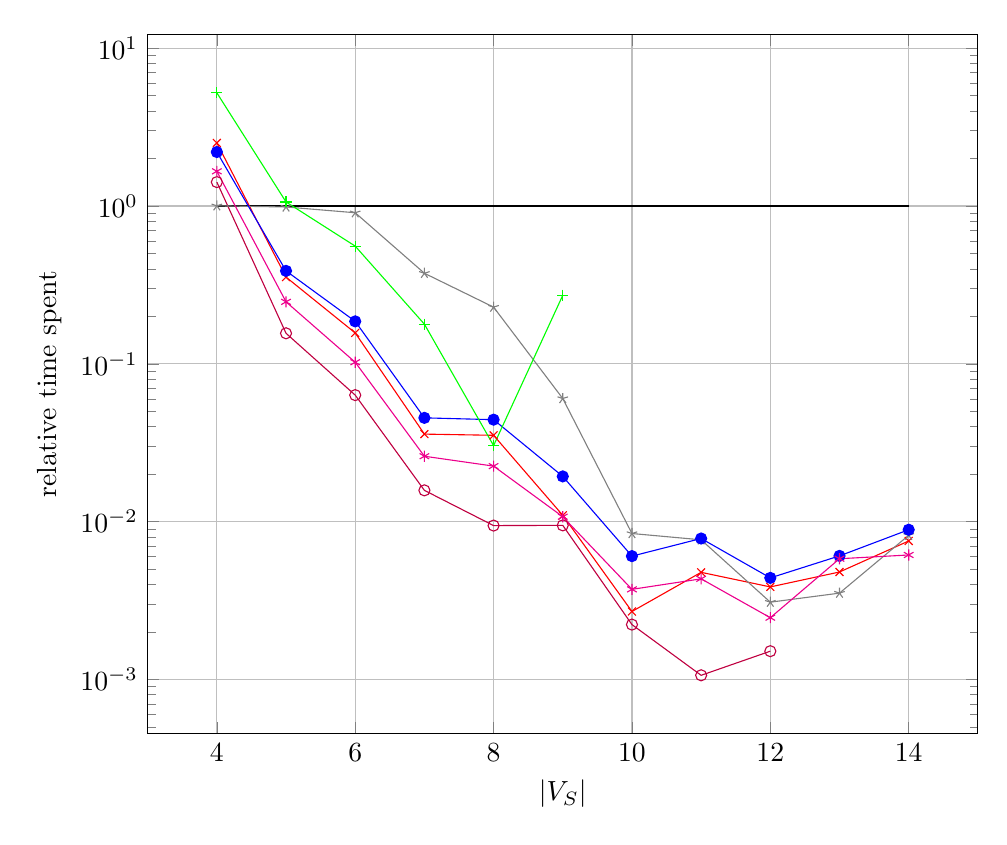
\begin{tikzpicture}
    \begin{axis}[
        xlabel=$|V_S|$,
        ylabel=relative time spent,
        ymode=log,
        legend style={at={(0.9,0.1)},anchor=south east},
        width=\textwidth,
		y tick label style={/pgf/number format/sci},
        ymajorgrids,
        xmajorgrids,		
    ]
\addplot [mark=none, black] plot coordinates {
        (4,1) (14, 1)};



\addplot[
        mark=x,
        red,
    ] plot coordinates {
        (4,2.5098178926779067)
        (5,0.3542854427484565)
        (6,0.15689010926635982)
        (7,0.035853449977087615)
        (8,0.03523223883158477)
        (9,0.010964699575333747)
        (10,0.0026948377810716018)
        (11,0.0047722023475749165)
        (12,0.003857850717237876)
        (13,0.0047953458790988)
        (14,0.007540380523948009)
};
%    \addlegendentry{DFS}


\addplot[
        mark=o,
        purple,
    ] plot coordinates {
        (4,1.4173101034075382)
        (5,0.1560990152619649)
        (6,0.06332634097438505)
        (7,0.0157805848059952)
        (8,0.009438491623514178)
        (9,0.009468907924155778)
        (10,0.002226287610086919)
        (11,0.001062190759533732)
        (12,0.0015102350651220453)
};
%    \addlegendentry{GDFS O IP}


\addplot[
        mark=star,
        gray,
    ] plot coordinates {
        (4,1.002529859429505)
        (5,0.9854105159518796)
        (6,0.906087246903251)
        (7,0.3747194523117736)
        (8,0.22865139116910282)
        (9,0.060236499046310454)
        (10,0.00840605207241163)
        (11,0.0076697916371780694)
        (12,0.003087366357886867)
        (13,0.003523082302813507)
        (14,0.008191107040264711)
};
%    \addlegendentry{GDFS C}


\addplot[
        mark=*,
        blue,
    ] plot coordinates {
        (4,2.1976489735425813)
        (5,0.3879928825633856)
        (6,0.18575151663949174)
        (7,0.0454443516390044)
        (8,0.044259974145741565)
        (9,0.01934413411554503)
        (10,0.006044262197985706)
        (11,0.007817157760072191)
        (12,0.004400728544806665)
        (13,0.0060658785631791945)
        (14,0.008884903299891778)
};
%    \addlegendentry{K-Path}


\addplot[
        mark=+,
        green,
    ] plot coordinates {
        (4,5.210336306845926)
        (5,1.0605278688734023)
        (6,0.5567531798646309)
        (7,0.17832988212555723)
        (8,0.03032795503714869)
        (9,0.2717523415218701)
};
%    \addlegendentry{CP}


\addplot[
        mark=asterisk,
        magenta,
    ] plot coordinates {
        (4,1.6585184570290825)
        (5,0.24696367603814495)
        (6,0.102320267871855)
        (7,0.025963378720697206)
        (8,0.02247569274863903)
        (9,0.010741035240163122)
        (10,0.003723269579006816)
        (11,0.004340017423267284)
        (12,0.0024617244953977213)
        (13,0.0058187731897781925)
        (14,0.006146499125306626)
};
%    \addlegendentry{GDFS A IP}

	
    \end{axis}
    \end{tikzpicture}

\caption{cached}

\end{subfigure}\\[1ex]
\begin{subfigure}{0.5\linewidth}
\centering

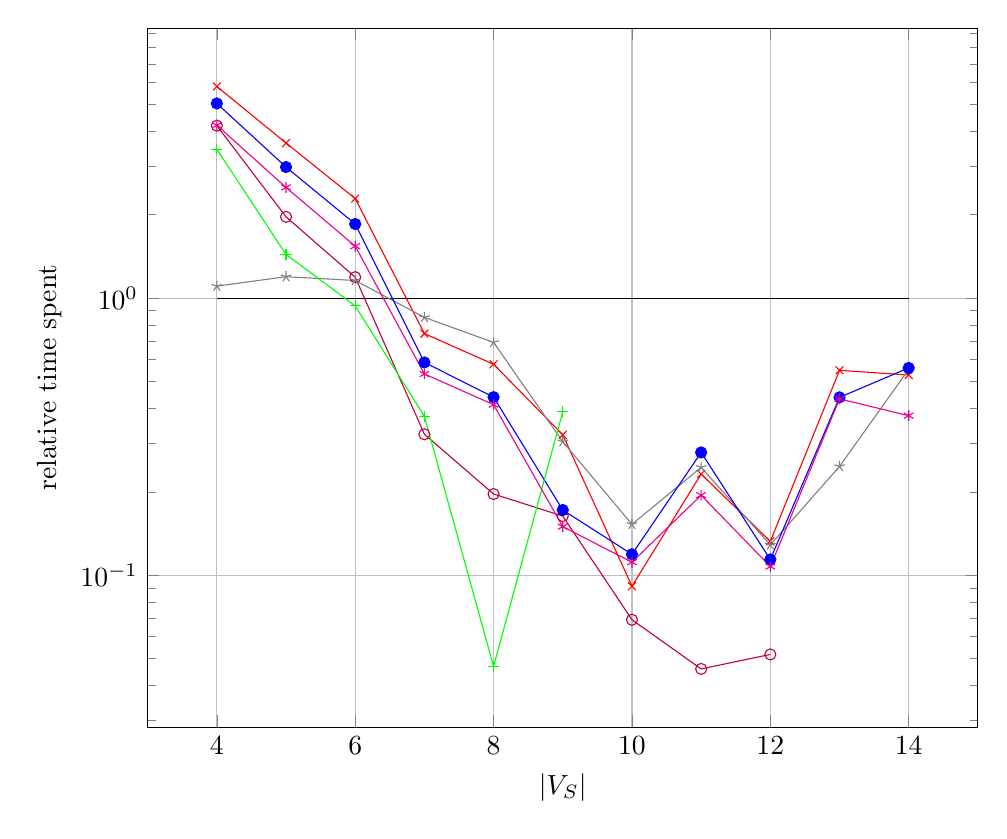
\begin{tikzpicture}
    \begin{axis}[
        xlabel=$|V_S|$,
        ylabel=relative time spent,
        ymode=log,
        legend style={at={(0.9,0.1)},anchor=south east},
        width=\textwidth,
		y tick label style={/pgf/number format/sci},
        ymajorgrids,
        xmajorgrids,		
    ]
\addplot [mark=none, black] plot coordinates {
        (4,1) (14, 1)};



\addplot[
        mark=x,
        red,
    ] plot coordinates {
        (4,5.798792679850153)
        (5,3.6257004403518205)
        (6,2.285202142417693)
        (7,0.7445129848838659)
        (8,0.5770188169893984)
        (9,0.3210938826132116)
        (10,0.09131787739629149)
        (11,0.23183733254071692)
        (12,0.13250978599133645)
        (13,0.5487572087616573)
        (14,0.5277236677256409)
};
%    \addlegendentry{DFS}


\addplot[
        mark=o,
        purple,
    ] plot coordinates {
        (4,4.1869563644643)
        (5,1.963563805539359)
        (6,1.1893882290176945)
        (7,0.3225915596294)
        (8,0.196417660886969)
        (9,0.1635088016201688)
        (10,0.06910862435318588)
        (11,0.045930260406800816)
        (12,0.0518105433910061)
};
%    \addlegendentry{GDFS O IP}


\addplot[
        mark=star,
        gray,
    ] plot coordinates {
        (4,1.1043656381381906)
        (5,1.1941146142677403)
        (6,1.1571769969713963)
        (7,0.8519147110949141)
        (8,0.6919890069549386)
        (9,0.30329744854481366)
        (10,0.15267006969696184)
        (11,0.2451122958148758)
        (12,0.12868565849738745)
        (13,0.2468665194487868)
        (14,0.5529525262522433)
};
%    \addlegendentry{GDFS C}


\addplot[
        mark=*,
        blue,
    ] plot coordinates {
        (4,5.036262260510419)
        (5,2.969188933770786)
        (6,1.8496830497872034)
        (7,0.5859718273323613)
        (8,0.43912493395440744)
        (9,0.17191408110115602)
        (10,0.11902810316960899)
        (11,0.2773735237523154)
        (12,0.114049211518233)
        (13,0.438365362697428)
        (14,0.5597451487697097)
};
%    \addlegendentry{K-Path}


\addplot[
        mark=+,
        green,
    ] plot coordinates {
        (4,3.4404078593966663)
        (5,1.4365332891311595)
        (6,0.9370666124380356)
        (7,0.37433319924673136)
        (8,0.04688253357281991)
        (9,0.38910890933793285)
};
%    \addlegendentry{CP}


\addplot[
        mark=asterisk,
        magenta,
    ] plot coordinates {
        (4,4.202135993006676)
        (5,2.5066991227985915)
        (6,1.5392306053079454)
        (7,0.5323918363219251)
        (8,0.41254854061922086)
        (9,0.14979269284608565)
        (10,0.11144241399443222)
        (11,0.1944784771207959)
        (12,0.10750387177004295)
        (13,0.43288906698477536)
        (14,0.37647551651848066)
};
%    \addlegendentry{GDFS A IP}

	
    \end{axis}
    \end{tikzpicture}

\caption{parallel}

\end{subfigure}
\begin{subfigure} {0.5\linewidth}
\centering

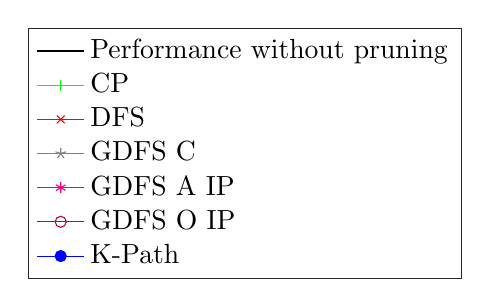
\begin{tikzpicture} 
    \begin{axis}[%
    hide axis,
    xmin=10,
    xmax=50,
    ymin=0,
    ymax=0.4,
    legend style={draw=white!15!black,legend cell align=left}
    ]
	\addlegendimage{black}
    \addlegendentry{Performance without pruning}; 
     
    \addlegendimage{green, mark=+}
    \addlegendentry{CP};
    
    \addlegendimage{red, mark=x}
    \addlegendentry{DFS};
    
    \addlegendimage{gray, mark=star}
    \addlegendentry{GDFS C};
    
    \addlegendimage{magenta, mark=asterisk}
    \addlegendentry{GDFS A IP};
    
    \addlegendimage{purple, mark=o}
    \addlegendentry{GDFS O IP};
    
    \addlegendimage{blue, mark=*}
    \addlegendentry{K-Path};
    
    \end{axis}
\end{tikzpicture}

\end{subfigure}

\caption{Performance of our algorithm with \textbf{AllDifferent} pruning using \textbf{`Labels and neighbours'} filtering relative to the performance of the algorithm without pruning. $|V_T|=1\frac{1}{2}*|V_S|$, ``refuse longer paths" and contraction are disabled and we use the degree-based target graph vertex ordering. Data points above the black reference line denote that the pruning method introduces more delay, and data points below the reference line denote that the pruning method saves time. Note the logarithmic y-axis.}	
\label{fig:alldifferentlabelsneighbours}
\end{figure}
